% 
%jff-notes
%
\documentclass[11pt]{article}
\usepackage[pdftex]{graphicx}
\usepackage{amssymb}
\usepackage{latexsym}
%\usepackage{relsize}
\usepackage{textcomp}
%processed for 10 pt 
%\documentstyle[epsf,psfig]{article}
%\documentstyle[epsf]{article}
\oddsidemargin 0pt
\topmargin -0.0cm
\textwidth 6.2in
\textheight 8.5in
\baselineskip 18pt
%\renewcommand{\baselinestretch} {1.5}
\newenvironment{nitemize}
   {\begin{list}{\begin{math}\bullet\end{math}}%
      {\setlength{\leftmargin}{5mm}
       \setlength{\topsep}{1mm}
       \setlength{\parsep}{0in}
       \setlength{\itemsep}{.7mm}}}%
   {\end{list}}

\newcommand{\fract}[2]{\frac{\textstyle #1}{\textstyle #2}}
\newcommand{\trans}[3]{#1 \stackrel{#2}{\longrightarrow} #3}
\newcommand{\notrans}[3]{#1 \stackrel{#2}{\not\! \longrightarrow} #3}
\bibliographystyle{plain}
\begin{document}
\title{A simple weatherfax plugin for SDRuno}
\author{
Jan van Katwijk\\
Lazy Chair Computing \\
The Netherlands\\
{\em J.vanKatwijk@gmail.com}}
%\date{}
\maketitle
%\baselineskip 22pt
\ \\
\ \\
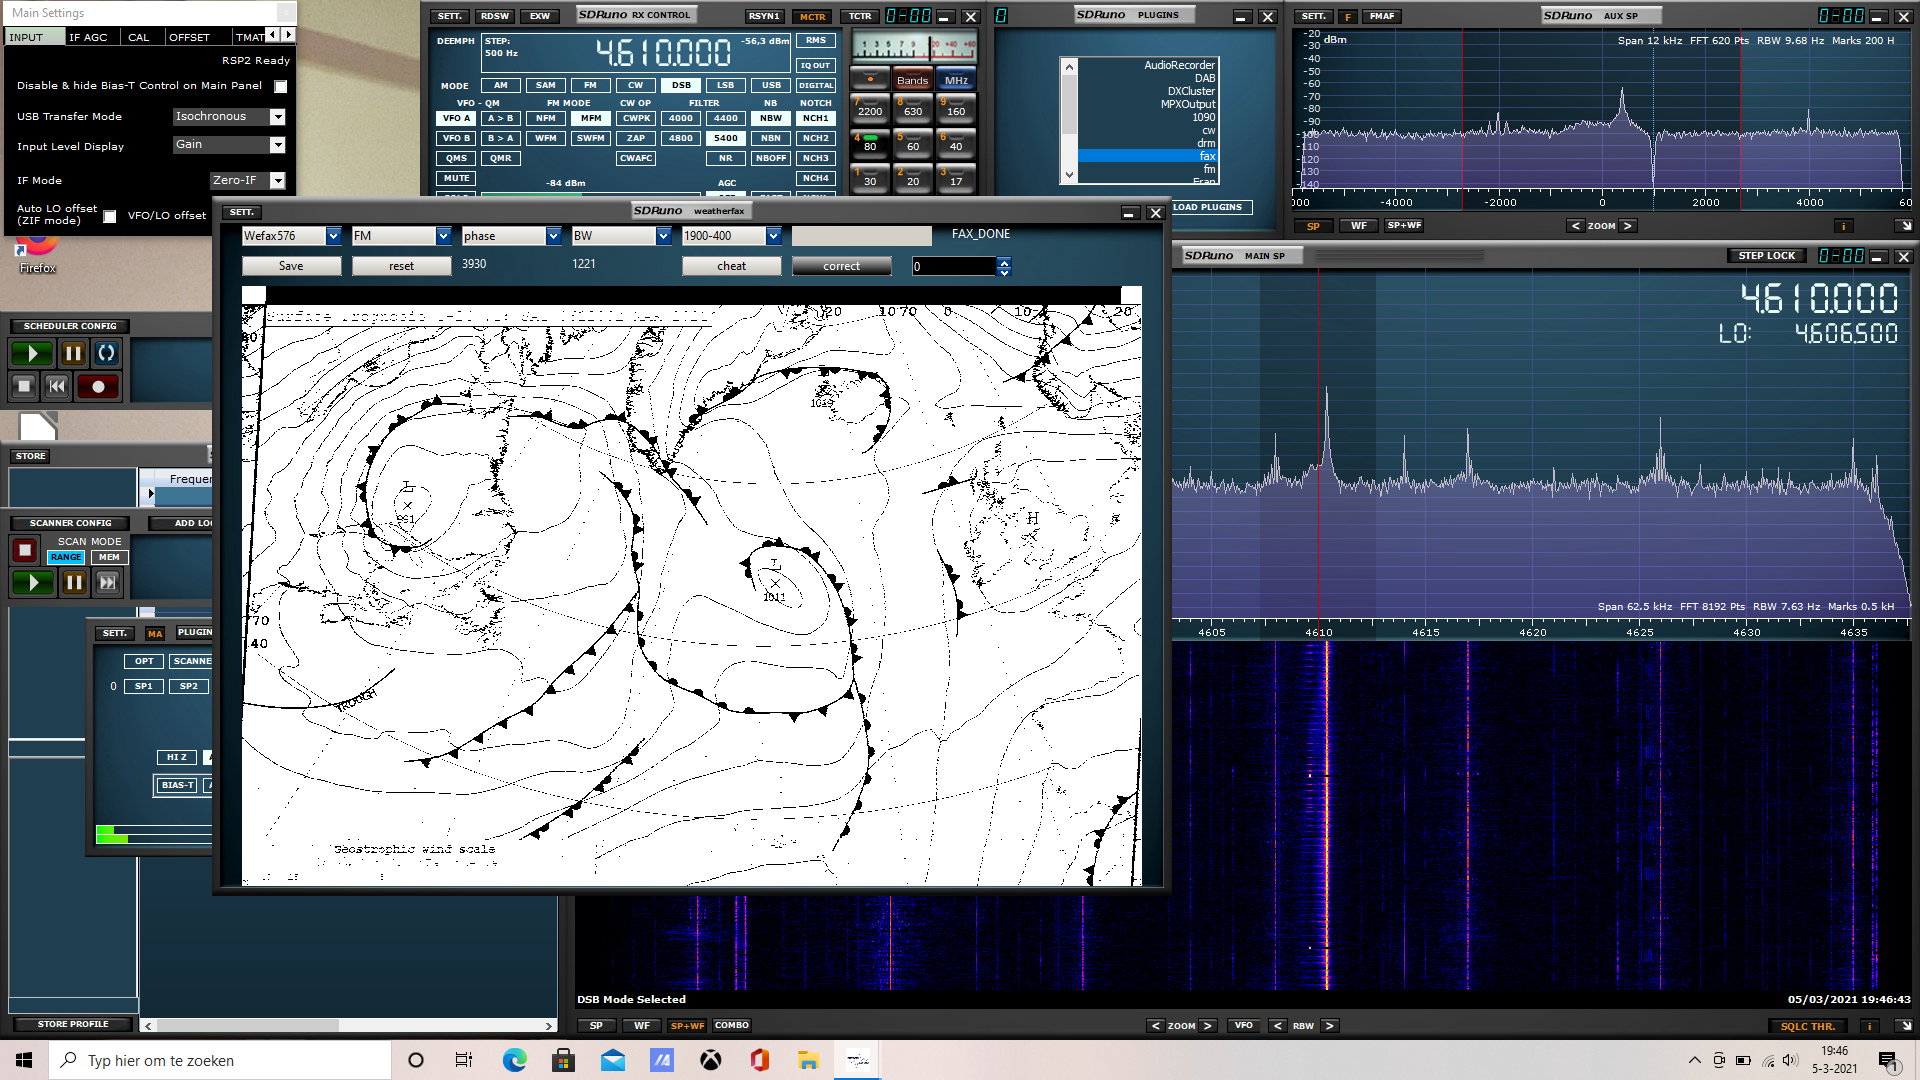
\includegraphics[width=150mm]{wfax-example.png}
\ \\
\section{Introduction}
The SDRuno weatherfax plugin is a simple plugin to decode weatherfax signals.

On shortwave (between 3 and 16 Mhz) there are
transmissions of weatherfax charts on a regular base.
Here, in western Europe, 3588 KHz and 4610 KHz are frequencies where
(almost) continuously weather charts are transmitted that can be received
(where I live people are extremely climate aware, so the number of
solar panels is overwhelming, and so is the amount of jamming signals,
from time to time making it virtually impossible
to receive a chart noise free).

The most common format for transmitting weather charts is
{\em Wefax576}, a format with an IOC (Index of Cooperation)
of 576 and 1200 lines charts.
The so-called IOC results in a width of the chart of
app 1800 pixels (the plugin reduces this to 900 pixels).

Transmission speed is 2 lines a minute, a chart has 1200 lines
so, with some header information preceding the chart, transmission
of a single chart takes more than 10 minutes.

Modulation of the signal is by phase shifting, with a signal deviation of
app  +400 Hz for white, and -400 Hz for black.

A transmission starts with a predefined signal, a few seconds, for Wefax576
precise 300 Hz,
followed by a number of {\em phase lines} with which the receiver can synchronize
with the transmission.
Such a {\em phase line} starts and ends with 2.5 \% of the linelength
with a pure white signal, and 95 \% of the linelength with pure black
(the picture of the chart shows in the top lines just a few of these
phase lines).

At the end of the transmission of a weatherchart, again, a tone
with predefined frequency is transmitted, just for a few seconds.
For Wefax576 this tone is at 450 Hz.

\section{SDRuno setting}
\subsection{Setting the samplerate}
The implementation uses a sample frequency of {\em 12 KHz},
similar to e.g. the navtex and the rtty plugin.
The SDRuno software can provide a samplerate
of 62.5 KHz, remaining filtering and decimation is done in
the weatherfax plugin itself.
The SDRuno setting is then to a samplerate of 2 MHz, and a decimation factor
32.

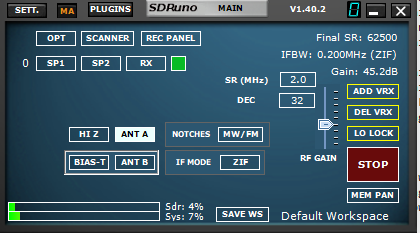
\includegraphics[width=100mm]{main-widget.png}

The plugin generates an audiotone of 800 Hz + the tuning offset,
so, when a transmission is active, two tones are heard, one for
white and one for black.

The sound is output with a rate of 48000, setting "AM" in the RX control window
will set this rate.

\subsection{Setting the frequency}

Transmission frequencies for weatherfax are predefined, so just select
a frequency from one of the lists of frequencies.
In 
\begin{verbatim}
https://www.weather.gov/media/marine/rfax.pdf
\end{verbatim}
one finds a list of stations.
\par
Note that - different from some other implementations - tuning is
{\em precisely} on the specified frequency, not 1900 Hz less!
\section{The plugin}
The widget for the plugin is shown in the picture below

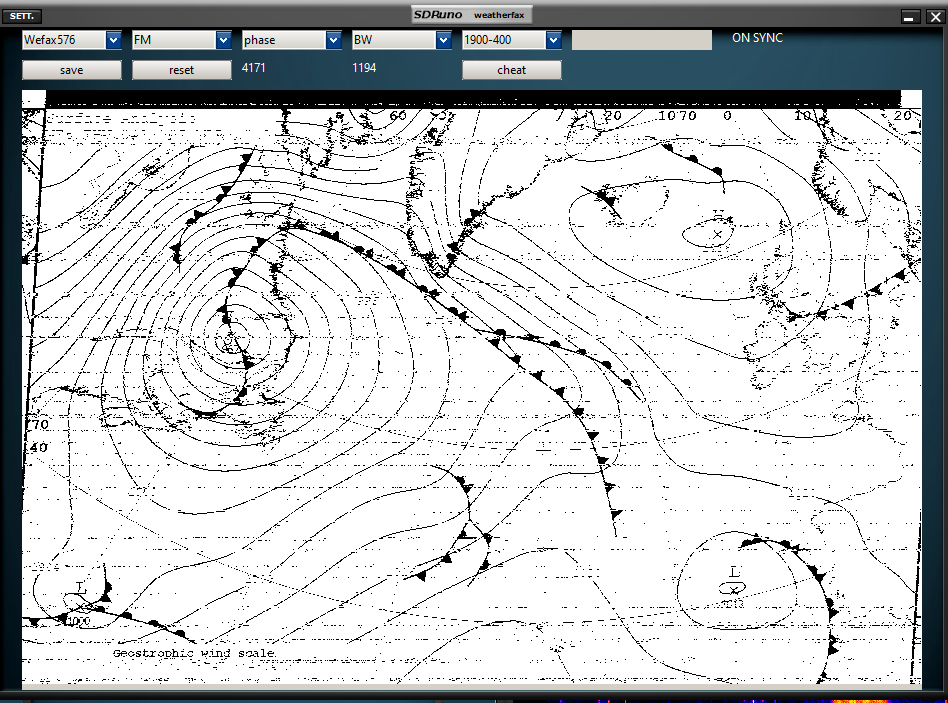
\includegraphics[width=140mm]{wfax-example-2.png}

The widget is large, the weather chart is displayed
on it. The size of the widget is such that a wefax576 chart is shown
on precisely one quarter of its size (app 900 pixels wide, 600 lines).
\par
The top two lines of the widget are reserved for the controls,
the {\em top one} contains (from left to right)
\begin{itemize}
\item a selector for the kind of charts, default Wefax576, alternatively
(but untested) Wefax288;
\item the {\em modulation mode}, default FM, alternatively AM;
\item the {\em phase}, by default the higher frequency of the signal
is used for {\em white}, the lower for {\em black}.
Selecting "invers" reverses this interpretation;
\item {\em BW}, a choice between Black and white, gray and color
(only black-white is used in the weathercharts and other settings are not
tested);
\item the {deviation}. While in Europe the deviation of the modulation is
400 Hz, literature states that the US uses 450 Hz.
\item a blank field (for later use);
\item a label displaying the {\em state} of the decoder. 
\begin{itemize}
\item {\em APTSTART} is - as the name suggests - the start state. The software
will read incoming signals until a few seconds a signal of 300 Hz
is received;
\item {\em PHASING} is the state where the software is trying to synchronize.
If - during a longer time - no reliable synchronization can be realized, the
asumtpion is that the detection of the 300 Hz was erroneous, and the APTSTART
state is entered;
\item {\em ON SYNC} is the state when a reliable synchronization is detected,
and in this state the data lines are processed.
The lines in the picture will be displayed on the widget.
\item {\em FAX\_DONE} is - as the name suggests - the stated entered when
processing the picture finishes. If {\em saving} was set, the picture
will be stored in a file and the APTSTART state will be entered again.
If {\em saving} was not set, the software will wait in the final state
until a {\em reset} is given.
\end{itemize}
\end{itemize}
The second line contains 8 elements
\begin{itemize}
\item the {\em save Cont} button. When set, the software will continuously
run the sequence to decode a picture and store each picture in a file.
The files are stored in the home filder of the user, and the name
will contain the time.
If set the text on the button shows as text {\em saving}, otherwise {\em Save}.
\item the {\em reset} button, which does what
can be expected from a reset button;
\item a label on which - while in the {\em APTSTART} state - the frequency
of the incoming decoded signal is displayed.
\item a label on which - when in sync - the line number
of the line currently being decoded is displayed;
\item a {\em cheat} button. As said, processing a whole chart in mode Wefax576
takes well over 10 minutes. The cheat button cheats the system by forcing
it into state {\em ON SYNC}. I.e. one can see some of the weatherchart,
even in the midddle of the transmission.
\item a {\em correct} button. Due to clock offsets,
the picture might be slightly leaning (as does the weatherchart on
the pictures).
When the picture is complete, it can be changed by touching this button.
The correction factor is then given in the spinbox to the right.
\item a {\em spinbox} telling the correction factor. Since the error is usually
small, the correction factor indicates the {\em amount of samples added
or subtracted from a group of 10 lines}. Experience shows that a correction of
"2" (i.e. 2 samples per 10 lines), will correct the picture.
\item a {\em save Single} button. After completing the decoding of a single
picture, the picture can be stored in a file.When selected, the
user will be requested to specify a filename.
\end{itemize}
\end{document}


